\documentclass{beamer}
\usetheme{STCE}

\usepackage{beamerfoils}
\usepackage[utf8]{inputenc}
\usepackage{amsmath}
\usepackage[german]{babel} % Für deutche Umlaute
\usepackage{tabularx} % Für die TabularX Umgebung

\MyLogo{
\centering

\includegraphics[width=0.12\textwidth]{./figures/logo.eps}
}

\begin{document}
\title{Correlation and Regression Analysis\\
TEACH}
\author{Patrick Neidig \and Marius Grysla}
\institute{Software and Tools for Computational Engeneering}
\date{31.5.2011}
\frame{\titlepage}

\begin{frame}
 \frametitle{Inhalt}
 \tableofcontents
\end{frame}

\section{Korrelation}
\begin{frame}
 
\end{frame}


\section{Multiple Regression}
\begin{frame}
 \frametitle{Das multiple lineare Regressionsmodell}
 \begin{itemize}
 \item Korrelationen:
   \begin{itemize}
   \item Verschiedene Merkmale haben einen Einfluß auf die Nettomiete
   \end{itemize}
 \item Offene Fragen:
   \begin{itemize}
   \item Mit welchem Aufpreis muss bei einer Wohnung in bester Wohnlage gerechnet werden?
   \item Hat das Baujahr einen Einfluss auf den Mietpreis/qm Verteilung?
   \end{itemize}
 \end{itemize}

 
\end{frame}



\begin{frame}
 \frametitle{Das multiple lineare Regressionsmodell}

 \begin{itemize}
  \item Wie groß sind die Einflüsse von verschiedenen Regressanden auf ein abhängiges Merkmal?
 \end{itemize}
 
 \begin{block}{Lineare Einfachregression}
  \begin{equation*}
   Y_i = \alpha + \beta x_i + \epsilon_i, \quad i = 1, \dots, n
  \end{equation*}
 \end{block}

 \begin{block}{Multiple Lineare Regression}
  \begin{equation*}
   Y_i = \beta_0 + \beta_1 x_{i1} + \dots + \beta_p x_{ip} + \epsilon_i, \quad i = 1, \dots, n
  \end{equation*}
  \begin{itemize}
   \item Anzahl der Regressanden: $p$
  \end{itemize}

 \end{block}

\end{frame}

\begin{frame}
  \frametitle{Verteilung Nettomieten}
  \begin{center}
    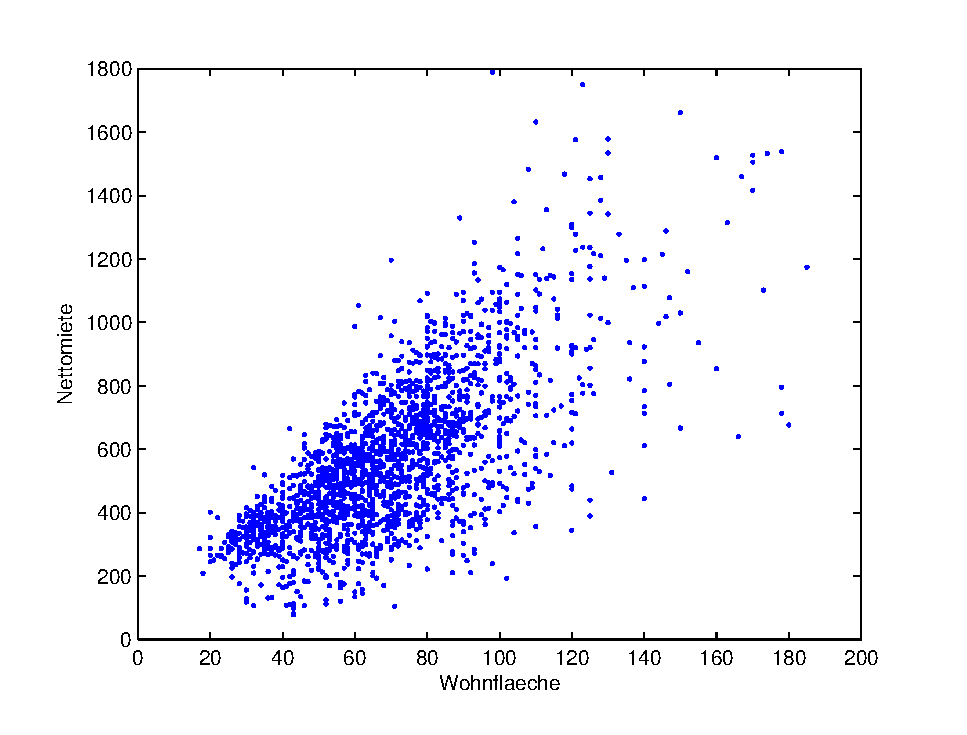
\includegraphics[width=10cm]{figures/nm_wfl_distribution}
  \end{center}
\end{frame}

\begin{frame}
  \frametitle{Verteilung Nettomieten II}
  \begin{center}
    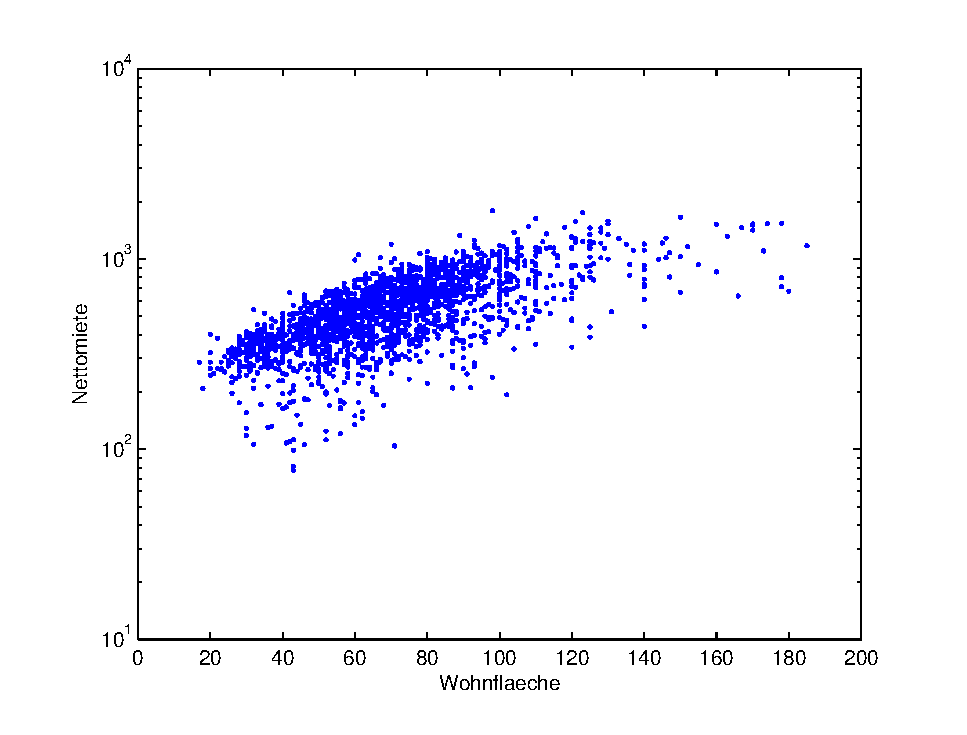
\includegraphics[width=10cm]{figures/nm_wfl_distribution_log}
  \end{center}
\end{frame}

\begin{frame}
  \frametitle{Anwendung}
  % Hier sollte die Verwendung der Regression mit dem Mietspiegel Beispiel verdeutlicht 
  
  % TODO: Welche Merkmale für Regression verwenden?
  %  - wohnfläche
  %  - wohnlage (gut, beste)
  %  - baujahr
  % TODO: Welche Zeilen auswählen

  \begin{itemize}
  \item Regressoren: Wohnfläche, gute Wohnlage, Baujahr
  \item Regressand: Nettomiete
  \end{itemize}

  \begin{block}{Regressionsansatz}
    \begin{equation*}
      log(NM) = \beta_0 + \beta_1 Wfl + \beta_2 Bj + \beta_3 gL + \epsilon
    \end{equation*}
  \end{block}

  % \begin{itemize}
  % \item Beispieldatensatz:\\
  %   \begin{tabular}[h]{c|c|c|c}
  %     1 & 2 & 3 & 4 \\
  %     5 & 6 & 7 & 8
  %   \end{tabular}
  % \end{itemize}

\end{frame}

\begin{frame}
  \frametitle{Funktionssignatur}
  
  \begin{itemize}
  \item Funktionsname: nag\_regsn\_mult\_linear (g02dac)
  \item Argumente:
    \begin{itemize}
    \item Anzahl der Beobachtungen $n$
    \item $m \times n$ Matrix $X$ mit den Beobachteten Werten für alle Variablen
    \item \dots
    \end{itemize}
  \end{itemize}

\end{frame}

\subsection{NAG Algorithmus}
\begin{frame}
  \frametitle{NAG Algorithmus}
 
  \begin{block}{Für Berechnung wird eine Matrixschreibweise benötigt}
    {\centering $y = X \beta + \epsilon$ \\}
    wobei \\
    \qquad $y$ = Vektor mit $n$ Beobachtungen von $y$ \\
    \qquad $X$ = Matrix mit den Beobachtungen der Regressanden \\
    \qquad $\beta$ = Vektor mit unbekannten Faktoren \\
    \qquad $\epsilon$ = Vektor mit Fehlertermen \\
  \end{block}
  
  \pause
  
  \begin{block}{Methode der kleinsten Quadrate}
    In Matrixschreibweise:\\
    {\centering
      $\sum\limits^{N}_{n=1} \epsilon^2_n = \epsilon^T \epsilon = (y - X \beta)^T (y - X \beta) \rightarrow \min\limits_{\beta}$\\}
    oder: \\
    {\centering
      $\Vert X\beta - y \Vert_2 \rightarrow \min\limits_{\beta}$
      \\}
  \end{block}

\end{frame}



\begin{frame}
  \frametitle{QR-Zerlegung}
  
  \begin{itemize}
  \item Wie kann das benötigte Minimum berechnet werden?\\
    $\Rightarrow$ QR-Zerlegung der Matrix $X$
  \end{itemize}

  \begin{block}{QR-Zerlegung}
    Zerlegung von $X$ in zwei Matrizen $Q$ und $R$, sodass \\
    \qquad $Q$ ist orthogonale Matrix \\
    \qquad $R$ enthält obere Dreiecksmatrix \\
  \end{block}

  \pause

  \begin{itemize}
  \item Algorithmen:
    % Hier Vor-/Nachteile erwähnen
    \begin{itemize}
    \item Householder Transformationen 
    \item Givens Rotationen 
    \item Modifizierter Gram-Schmidt Algorithmus 
    \end{itemize}
  \end{itemize}

\end{frame}

\begin{frame}
  \frametitle{Householder Verfahren}
  \begin{block}{Householder Matrix}
    \[ P = I - 2vv^T / v^Tv \]    
    \begin{itemize}
    \item Erzeugt in einer Spalte $x$ Nullen
    \end{itemize}
  \end{block}
  
  \begin{itemize}
  \item Berechnung von $v$:\\
    $v = x / \beta,$\hspace{1cm} $v(1) = 1$ \\
    $\beta = x(1) + sign(x(1)) \|x\|_2$
  \end{itemize}

\end{frame}

\begin{frame}
  \frametitle{QR-Zerlegung (Beispiel)}
  $X = \small \begin{pmatrix}
    1	& 36	& 1948	& 0 \\
    1	& 65	& 1966	& 0 \\
    1	& 79	& 1986	& 1 \\
    1	& 93	& 1918	& 1 \\
    1	& 102	& 1918	& 0 \\
    1	& 121	& 1924	& 1 \\
    1	& 128	& 1991	& 1 \\
    1	& 150	& 1966	& 0 
  \end{pmatrix},$
  $x = \small \begin{pmatrix}
    1 \\ 1 \\ 1 \\ 1 \\ 1 \\ 1 \\ 1 \\ 1
  \end{pmatrix},$ 
  \pause
  $\beta = 3.83,$
  $v = \begin{pmatrix}
    1.00 \\ 0.26 \\ 0.26 \\ 0.26 \\ 0.26 \\ 0.26 \\ 0.26 \\ 0.26
  \end{pmatrix}$ \\

  \pause
  
  $(I - 2vv^T/v^Tv) X = \small \begin{pmatrix}
    -2.83 & -273.65 & -5521.44 & -1.41 \\
    0 & -15.88 & 14.95 & -0.37 \\
    0 &	-1.88 &	34.95 &	0.63 \\
    0 &	12.12 & -33.05 & 0.63 \\
    0 & 21.12 &	-33.05 & -0.37 \\
    0 &	40.12 & -27.05 & 0.63 \\
    0 &	47.12 &	39.95 & 0.63 \\
    0 & 69.12 & 14.95 & -0.37 
  \end{pmatrix}$
\end{frame}

\begin{frame}
  \frametitle{QR-Zerlegung (Beispiel) II}
  $\underbrace{P_4 P_3 P_2 P_1 X}_{R} = \footnotesize \begin{pmatrix}
    -2.83 & -273.65 & -5521.44 & -1.41 \\
    0 & 97.24 & 4.41 & 0.35 \\
    0 & 0 & -78.49 & -0.11 \\
    0 & 0 & 0 & -1.37 \\
    0 & 0 & 0 & 0 \\
    0 & 0 & 0 & 0 \\
    0 & 0 & 0 & 0 \\
    0 & 0 & 0 & 0 \\
  \end{pmatrix}$
  
  \vspace{1cm}
  \pause

  $\underbrace{P_1  P_2  P_3  P_4}_{Q} = \nobreak
  \footnotesize
  \begin{pmatrix}
    0.25 & -0.62 & -0.02 & -0.20 & -0.08 & 0.26 & 0.52 & 0.31 \\
    0.35 & -0.33 & 0.20 & -0.30 & -0.14 & 0.21 & -0.56 & -0.51 \\
    0.35 & -0.18 & 0.44 & 0.38 & 0.17 &	-0.42 &	-0.32 &	0.44 \\
    0.35 & -0.04 & -0.43 & 0.41 & -0.54 & -0.37 & 0.12 & -0.27 \\
    0.35 & 0.05 & -0.44 & -0.34 & 0.63 & -0.38 & 0.02 & -0.11 \\
    0.35 & 0.25 & -0.37 & 0.33 & 0.15 & 0.63 & -0.27 & 0.26 \\
    0.35 & 0.32 & 0.48 & 0.24 & 0.23 & 0.15 & 0.47 & -0.43 \\
    0.35 & 0.55 & 0.15 & -0.52 & -0.42 & -0.09 & 0.01 & 0.32 
  \end{pmatrix}$
\end{frame}

\begin{frame}
  \frametitle{Gleichungssystem Lösen}
  
  \begin{itemize}
  \item Wir haben: $X = QR^*$, wobei $R^* = \binom{R}{0}$
  \item Es gilt: $\Vert X\beta - y \Vert_2 = \Vert Q^T X \beta - Q^T y \Vert_2 = \Vert R \beta - c \Vert_2 + \Vert d \Vert_2$
  \item $Q^T * y = \binom{c}{d}$
  \item Löse $R \hat{\beta} = c$ durch Rückwärtseinsetzen

  \pause

  \item Funktioniert nur bei vollem Rang von $R$!
  \end{itemize}

\end{frame}

\begin{frame}
  \frametitle{Gleichungssystem Lösen (Beispiel)}
  \begin{itemize}
  \item $c$ berechnen: \\ 
    $Q^T * log NM = $
    $Q^T * \scriptsize \begin{pmatrix} 5.37 \\ 6.01 \\ 6.40 \\ 6.72 \\ 6.91 \\ 7.11 \\ 7.23 \\ 7.42 \end{pmatrix} = $
    $\scriptsize \begin{pmatrix} 18.80 \\ 1.79 \\ -0.14 \\ 0.20 \\ 0.16 \\ -0.17 \\ -0.06 \\ -0.11 \end{pmatrix}$
    % TODO: Ist es möglich rechts eine Klammer um die Werte von c zu machen?

    \pause

  \item Lösen: \\
    $R * \begin{pmatrix} \beta_0 \\ \beta_1 \\ \beta_2 \\ \beta_3 \end{pmatrix} = \begin{pmatrix} 18.80 \\ 1.79 \\ -0.14 \\ 0.2 \end{pmatrix}$
    \pause
    $\Rightarrow \begin{pmatrix} \beta_0 \\ \beta_1 \\ \beta_2 \\ \beta_3 \end{pmatrix} = \begin{pmatrix} 8.63 \\ 0.02 \\ -0.002 \\ 0.15 \end{pmatrix}$
  \end{itemize}
  \end{frame}

\begin{frame}
  \frametitle{Ergebnis}
  \begin{block}{Regressionsansatz}
    \centering
    $ log(NM) = \alt<2->{\alert<2>{8.68}}{\beta_0} + \alt<2->{\alert<2>{0.02}}{\beta_1} Wfl \alt<2->{\alert<2>{- 0.002}}{+ \beta_2} Bj + \alt<2->{\alert<2>{0.15}}{\beta_3} gL + \epsilon $
      \pause\pause
    \[ \Rightarrow NM = exp(8.68) exp(0.02 Wfl) exp(-0.002 Bj) exp(0.15 gL) \]
        
  \end{block}

  \pause

  \begin{itemize}
  \item $NM = NM_B \alpha$
  \item Basismiete: \\
    $NM_B = 5619 \times exp(0.02 Wfl) exp(-0.002 Bj)$ \\
    \only<5>{\alert{$NM_B = 0.059 \times exp(0.012 Wfl) exp(0.004 Bj)$}}
  \item Zuschlag: \\
    $\alpha = exp(0.146) = 1.158$ \\
    \only<5>{\alert{$\alpha = exp(0.105) = 1.111$}}
  \end{itemize}
\end{frame}

\begin{frame}
  \frametitle{Ergebnis II}
  % Plots mit Mieten im Verhältnis zu Regressoren zeigen
  % Ergebnis der Beispielrechnung mit dem Regressionsergebnis mit vollständigen Daten vergleichen. 
  \begin{center}
    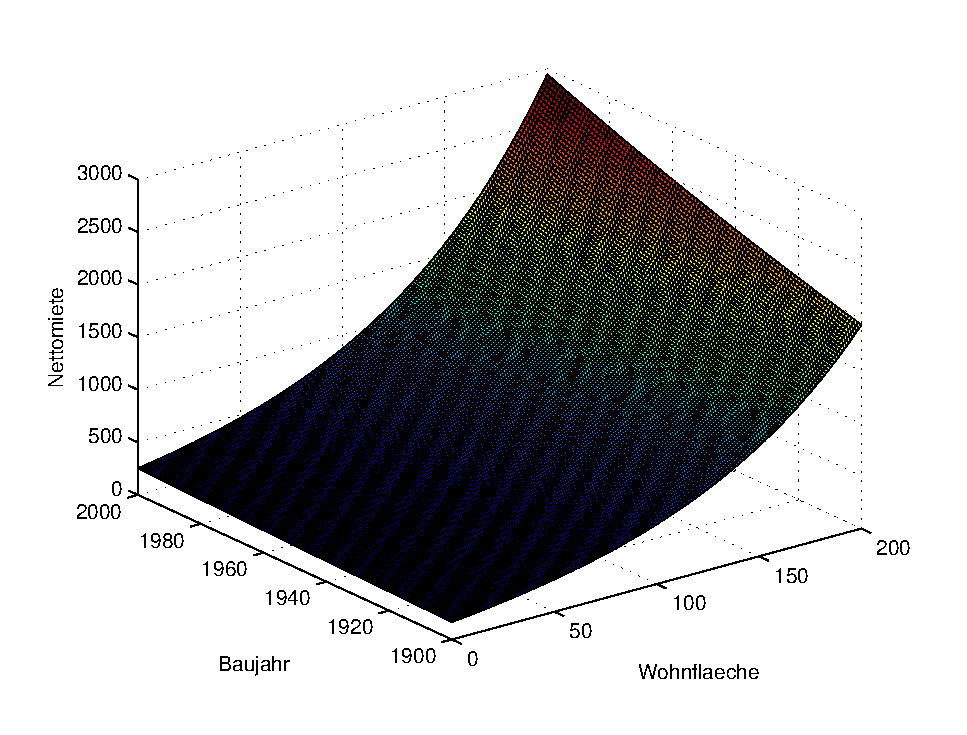
\includegraphics[width=10cm]{figures/nm_wfl_bj_log_approach}
  \end{center}

\end{frame}

\begin{frame}
  \frametitle{Ausblick}
  
  Im nächsten Vortrag folgt:
  \begin{itemize}
  \item Wie werden die Methoden angewendet
    \begin{itemize}
    \item Am Beispiel des Münchener Mietspiegels
    \end{itemize}
  \item Performance Analyse
    \begin{itemize}
    \item Wie verhalten sich die Algorithmen bei verschiedenen Datensätzen/Parametern 
    \end{itemize}
  \end{itemize}

\end{frame}

\end{document}
